\subsection{Shifting Event Positions to GRB position}
\label{sec:shift2source}
In later steps the directions of different neutrino events will be compared to
each other. Therefore, all events within a zenith band need to be shifted such
that their true
direction $\vec{t}$ will coincide with the GRB direction $\vec{g}$ and the
shifted or new reconstructed direction $\vec{n}$ should have the same distance
and direction
to $\vec{g}$ as the originally reconstructed direction $\vec{r}$ had to
$\vec{t}$.

The following calculations will be made in cartesian coordinates by
transforming the zenith and azimuth angle
\begin{equation}
 \begin{align}
  x &= \text{sin}\theta \cdot \text{cos} \phi \\
  y &= \text{sin}\theta \cdot \text{sin} \phi \\
  z &= \text{cos}\theta\\
 \end{align}
\end{equation}
with $\phi \in [0, 2 \pi)$, $\theta \in [0, \pi]$
The angular difference between $\vec{t}$ and $\vec{r}$ is
\begin{equation}
 \text{cos} \alpha = \frac{\vec{r} \cdot \vec{t}}{|\vec{r}| |\vec{t}|}
\end{equation}
and the direction of $\vec{r}$ relative to $\vec{t}$ is
\begin{equation}
 \vec{e} = \frac{\vec{r} - \vec{t}}{|\vec{r} - \vec{t}|}
\end{equation}
Therefore, the following conditions need to be met
\begin{align}
 \text{cos} \alpha &= \frac{\vec{r} \cdot \vec{t}}{|\vec{r}| |\vec{t}|} =
\frac{\vec{n} \cdot \vec{g}}{|\vec{n}| |\vec{g}|} \\
\vec{n} & = \vec{g} + c \vec{e}
\end{align}
leaving the factor c to be the only unkown to determine $\vec{n}$. There should
be two solutions, one in the positive and one in the negative direction
yealding two possible vectors that fullfill the same angular distance to the GRB
direction $\vec{g}$. As $\vec{e}$ points into the intended direction, $c$ will
be always chosen as positive.

Combining the conditions, one can derive the factor $c$
\begin{equation}
\label{eq:ang_dist_shifting}
 \begin{align}
 \text{cos} \alpha &= \frac{\vec{n} \cdot \vec{g}}{|\vec{n}| |\vec{g}|} \\
&= \frac{\left(\vec{g} + c \vec{e} \right) \cdot \vec{g}}{|\vec{g} + c
\vec{e}| |\vec{g}|} \\
&= \frac{\left(g_x + c \cdot e_x\right) \cdot g_x + \left(g_y + c \cdot
e_y\right) \cdot g_y + \left(g_z + c \cdot e_z\right) \cdot
g_z}{\sqrt{\left(g_x + c e_x \right)^2 + \left(g_y + c e_y \right)^2 +\left(g_z
+ c e_z \right)^2 } \cdot \sqrt{g_x^2 + g_y^2 +g_z^2}} \\
&= \frac{g_x^2 + g_y^2 +g_z^2 + c \cdot \left(e_x g_x + e_y g_y + e_z g_z
\right)}{\sqrt{g_x^2 + g_y^2 +g_z^2 + 2 c \cdot \left(e_x g_x + e_y g_y + e_z
g_z \right) + c^2 \left( e_x^2 + e_y^2 + e_z^2 \right) } \cdot \sqrt{g_x^2 +
g_y^2 +g_z^2}} \\
&= \frac{\gamma + c \cdot \tau}{\sqrt{\gamma + 2 c \cdot \tau + c^2 \cdot \zeta}
\sqrt{\gamma}}
 \end{align}
\end{equation}
with the abbreviations
\begin{equation}
 \begin{align}
  \gamma &= \vec{g}^2 = g_x^2 + g_y^2 +g_z^2 \\
  \tau &= \vec{g}\cdot \vec{e}=e_x g_x + e_y g_y + e_z g_z\\
  \zeta &=  \vec{e}^2 =e_x^2 + e_y^2 + e_z^2
 \end{align}
\end{equation}
Calculating the square of equation \ref{eq:ang_dist_shifting} and rewriting it
to fit the
standard p,q - formulism, one obtains
\begin{equation}
 \begin{align}
\left(
\gamma + 2 c \cdot \tau + c^2 \cdot \zeta \right) \gamma \cdot \text{cos}^2
\alpha - \left(\gamma^2 + 2 c \tau \gamma  + c^2 \tau^2 \right) &= 0\\
\text{cos}^2\alpha \left(\gamma^2 + 2 c \cdot \tau \gamma + c^2 \cdot \zeta
\gamma \right) - \left( \gamma^2 + 2 c \tau \gamma  + c^2 \tau^2\right) &= 0\\
c^2 \cdot \left(\zeta \gamma \text{cos}^2\alpha - \tau^2 \right) + 2 c \cdot
\tau \gamma \left( \text{cos}^2\alpha - 1 \right) + \gamma^2 \left(
\text{cos}^2\alpha - 1 \right)  &= 0 \\
c^2 + c \cdot \frac{ 2 \tau \gamma \left(\text{cos}^2\alpha - 1 \right)}{\zeta
\gamma \text{cos}^2\alpha - \tau^2} + \frac{\gamma^2 \left(
\text{cos}^2\alpha - 1 \right) }{\zeta
\gamma \text{cos}^2\alpha - \tau^2} &= 0 \\
c^2 + p \cdot c + q &= 0
%  \end{align}
%  \begin{align}
 \end{align}
\end{equation}
Therefore, $c$ has two solutions as predicted. The positive will always be
chosen.
\begin{equation}
 c = -  \frac{\tau \gamma \left(\text{cos}^2\alpha - 1 \right)}{\zeta
\gamma \text{cos}^2\alpha - \tau^2} \pm \sqrt{\left( \frac{\tau \gamma
\left(\text{cos}^2\alpha - 1 \right)}{\zeta
\gamma \text{cos}^2\alpha - \tau^2} \right)^2 - \frac{\gamma^2 \left(
\text{cos}^2\alpha - 1 \right) }{\zeta
\gamma \text{cos}^2\alpha - \tau^2}}
\end{equation}

The value of c leads to the calculation of the new reconstructed direction
$\vec{n}$ which can be transformed back into spherical coordinates using
\begin{equation}
 \theta = \text{arccos} \left( \frac{n_z}{|\vec{n}|} \right)
\end{equation}
\begin{equation}
 \begin{align}
  \phi &= \text{arctan} \left( \frac{n_y}{n_x}\right)  \text{,  if  } n_x > 0\\
  \phi &= sign \left(n_y \right) \cdot \frac{\pi}{2}  \text{,  if  } n_x = 0\\
  \phi &= \text{arctan} \left( \frac{n_y}{n_x}\right) + \pi  \text{,  if  } n_x
<0 \text{ and } n_y \geq 0\\
  \phi &= \text{arctan} \left( \frac{n_y}{n_x}\right) - \pi  \text{,  else}\\
 \end{align}
\end{equation}


% \begin{framed}
% There are very few events for which this is
% not true. The reason is unknown at this moment. 
% \end{framed}
 


 
\begin{figure}[htbp]
  \centering
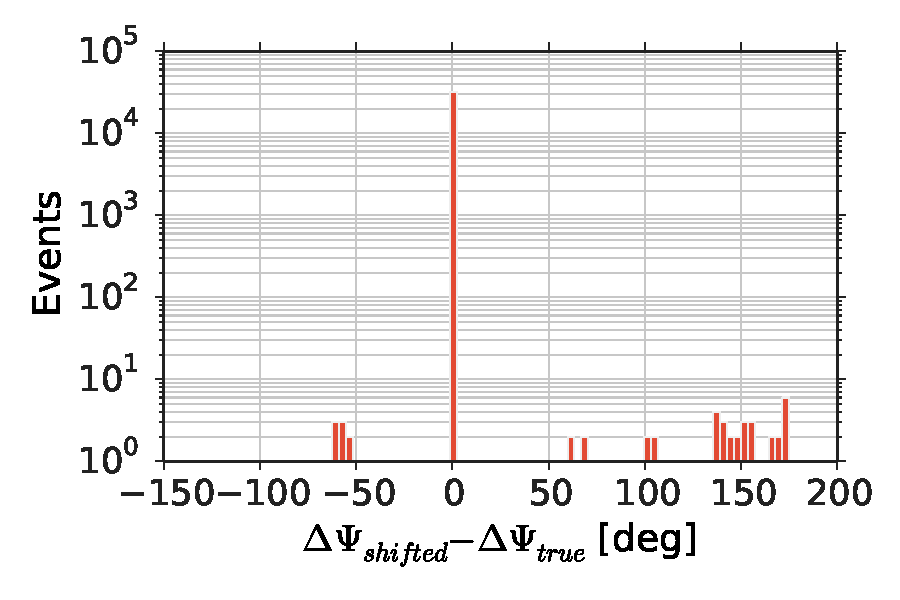
\includegraphics[width=
1.\textwidth]{fig/shift2source_true_minus_shifted_error.pdf}
  \caption{\label{fig:shift2source_proof}Shown is the difference between the
true error between reconstructed and true direction and the error between the
shifted reconstructed direction and the GRB direction. Almost all events have 
been shifted perfectly.}
\end{figure}

\begin{figure}[h]
\centering
 \captionsetup{width=.9\textwidth}
%  \captionsetup{margin=0pt}
\subfloat[Dependency on zenith angle.\label{fig:shift2source_zendependency}]{%
 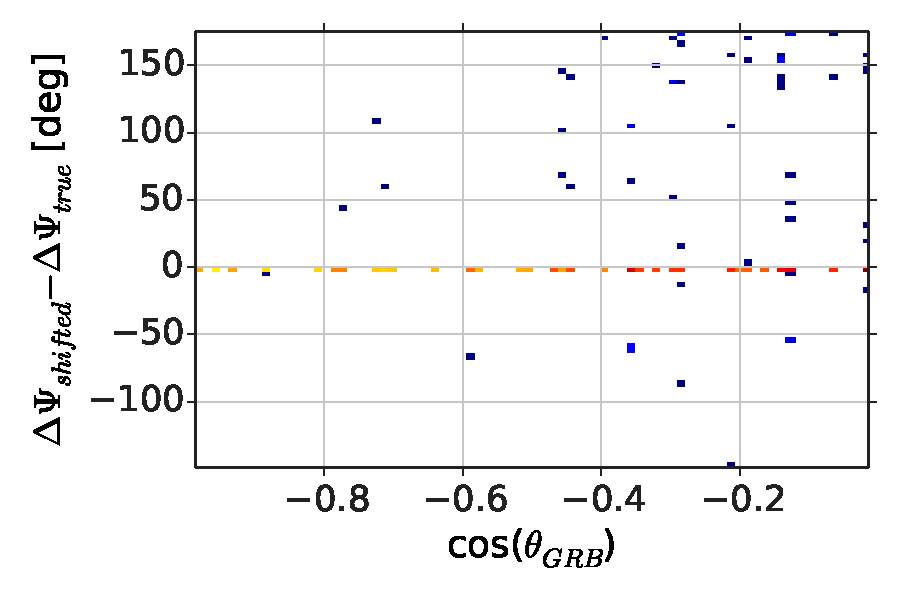
\includegraphics[width=0.45\textwidth]{fig/shift2source_zendependency.pdf}}
 \subfloat[Dependency on the azimuth angle. 
\label{fig:shift2source_azidependency}]{%
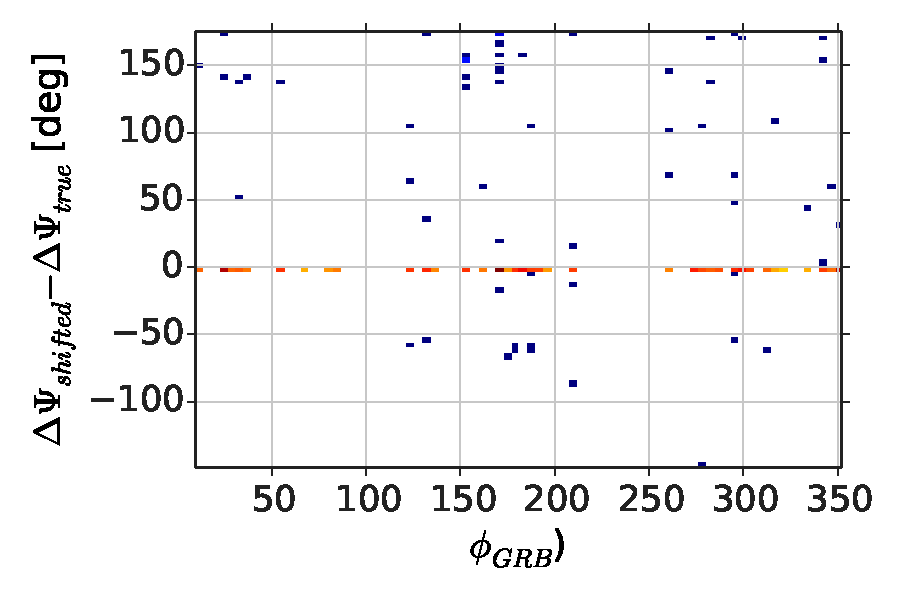
\includegraphics[width=0.45\textwidth]{fig/shift2source_azidependency.pdf}}
\caption{Two dimensional histograms showing the dependency of the difference 
between shifted and true reconstruction error to the zenith (left) and azimuth 
angle (right). No true dependency can be seen.}
\end{figure}

Figure \ref{fig:shift2source_proof} demonstrates that, for almost all events, 
the new directions 
have
 the same distance to the GRB as the originally
reconstructed directions had compared to their true directions. There are few 
events \textbf{(I need a percentage here!!!???)} for which the process doesn't 
work. The reasons are unknown at this point. Figures 
\ref{fig:shift2source_zendependency} and \ref{fig:shift2source_azidependency} 
demonstrate that there is no directional correlation. However, as this effect 
is only true for ???\% of the events, the effect can be neglected.
% An example skymap for one GRB and the correspondingly shifted neutrino
% directions is shown in Figure \ref{fig:skymap_grb}.